\documentclass{article}
\usepackage[utf8]{inputenc}
\usepackage{graphicx}
\usepackage{ragged2e}
\usepackage[margin=2.5cm]{geometry}
\usepackage{array}
\usepackage{wrapfig}
\usepackage{multirow}
\usepackage{tabularx}
\usepackage{amsmath}
\usepackage{wrapfig}
\usepackage{gensymb}
\usepackage{mathtools}
\usepackage[table]{xcolor}
\usepackage{multirow}
\usepackage{polski}
\usepackage{rotating}
\title{Charakterystyka czasowa}
\author{Marcin Gruchała 248982\\
Jan Bronicki 249011\\}
\date{}


\begin{document}
\maketitle
\section{Cel ćwiczenia.}
Badanie charakterystyk czasowych, dla różnych równań
\section{Rozwiązanie analityczne równania różniczkowego i jego wykres.}
$$
\ddot{x}(t)+\dot{x}(t)-2x(t)=u(t), u(t)=1, \dot{x}(0)=0, x(0)=2
$$
Rozwiązanie swobodne:
$$
\ddot{x}_s(t)+\dot{x}_s(t)-2x_s(t)=0
$$
$$
x_s(t)=Ae^{\lambda t}, \dot{x}_s(t)=\lambda Ae^{\lambda t}, \ddot{x}_s(t)=\lambda^2 Ae^{\lambda t}
$$
$$
\lambda^2 Ae^{\lambda t}+\lambda Ae^{\lambda t}-2Ae^{\lambda t}=
0/:Ae^{\lambda t}
$$
$$
\lambda^2+\lambda-2=0
$$
$$
\Delta=9, \lambda_1=-2, \lambda_2=1
$$
$$
x_s(t)=A_1e^{-2t}+A_2e^{t} - \text{rozwiązanie swobodne}
$$
Rozwiązanie wymuszone:
$$
\ddot{x}_w(t)+\dot{x}_w(t)-2x_w(t)=1
$$
$$
u(t)=1,\dot{u}(t)=0 ,\ddot{u}(t)=0
$$
$$
x_w(t)=C_1\cdot1+C_2\cdot0+C_3\cdot0
$$
$$
\dot{x}_w(t)=0,\ddot{x}_w(t)=0
$$
$$
-2C_1=1 \Rightarrow C_1=-\frac{1}{2} \Rightarrow X_w(t)=-\frac{1}{2} - \text{rozwiązanie wymuszone}
$$
Rozwiązanie ogólne: 
$$
x(t)=x_s(t)+x_w(t)
$$
$$
x(t)=A_1e^{-2t}+A_2e^{t}-\frac{1}{2}-\text{rozwiązanie ogólne}
$$
Rozwiązanie szczególne:
$$
x(t)=A_1e^{-2t}+A_2e^{t}
$$
$$
\dot{x}(t)=-2A_1e^{-2t}+A_2e^{t}
$$
$$
x(0)=A_1+A_2-\frac{1}{2}=2
$$
$$
\dot{x}(0)=-2A_1+A_2=0
$$
$$
A_1=\frac{A_2}{2}
$$
$$
\frac{A_2}{2}+A_2-\frac{1}{2}=2 \Rightarrow A_2=\frac{5}{3}=\frac{10}{6}
\Rightarrow A_1=\frac{5}{6}
$$
$$
x(t)=\frac{5}{6}e^{-2t}+\frac{10}{6}e^{t}-\frac{1}{2}-\text{rozwiązanie szczególne}
$$
\newpage
Wykres:
\begin{figure}[h!]
    \centering
     \begin{turn}{270}
    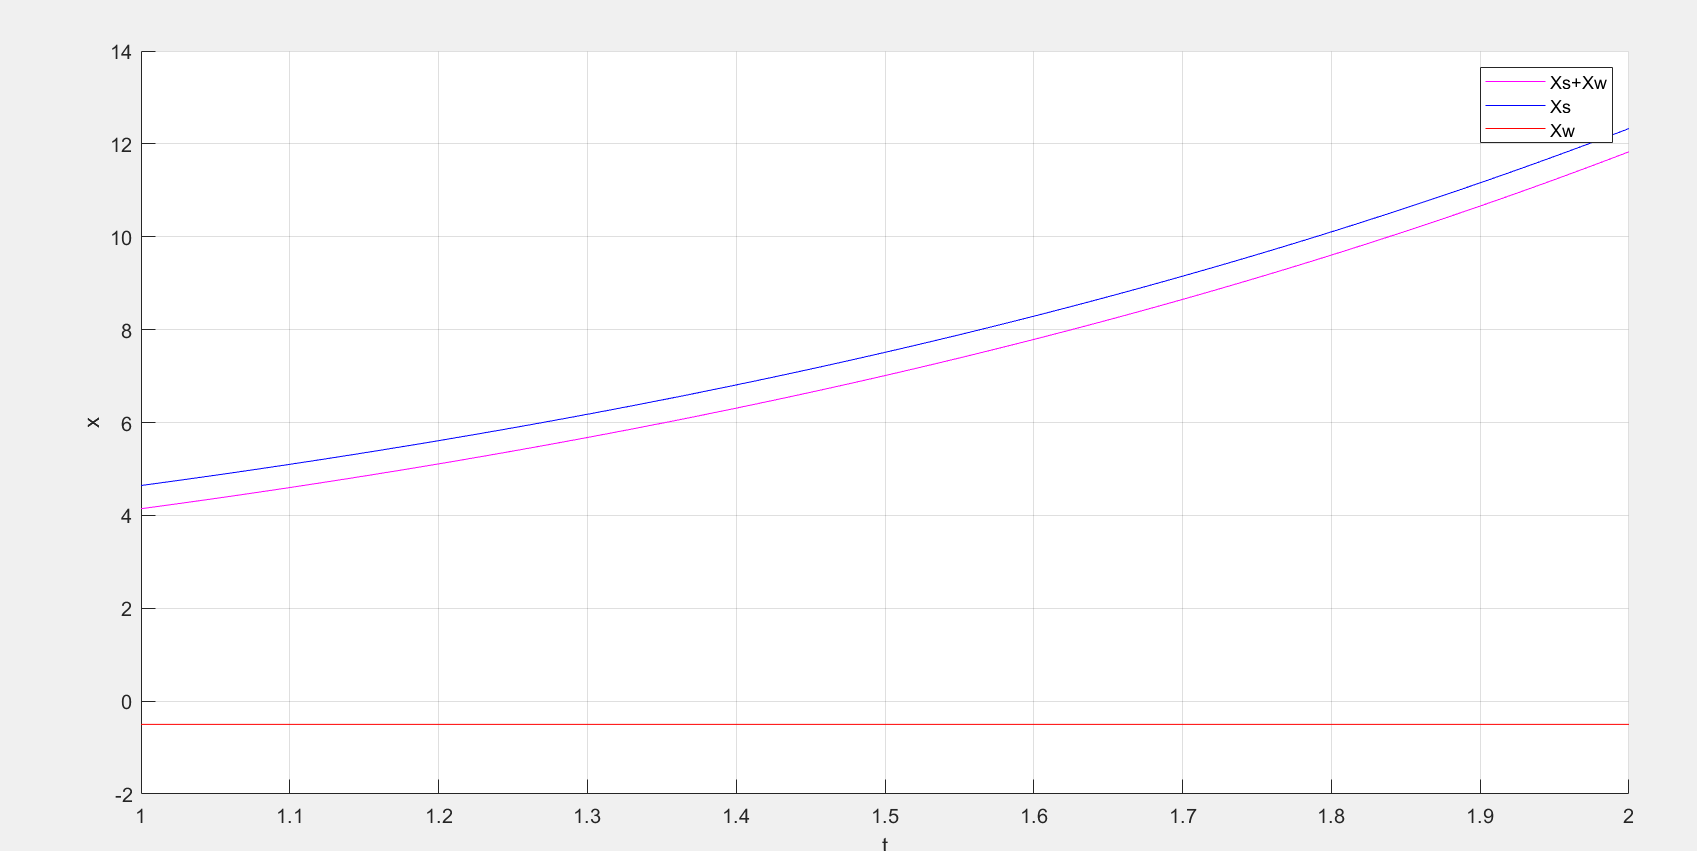
\includegraphics[width=1.3\textwidth]{rozwiazanie_analityczne_wykres.png}
    \end{turn}
    \label{fig:my_label}
\end{figure}


\newpage
\section{Badanie wpływu parametrów.}
\subsection{$A,\alpha,x_0$}
$$
x(t)=Ae^{\alpha t}+x_0
$$

\begin{figure}[h]
    \centering
    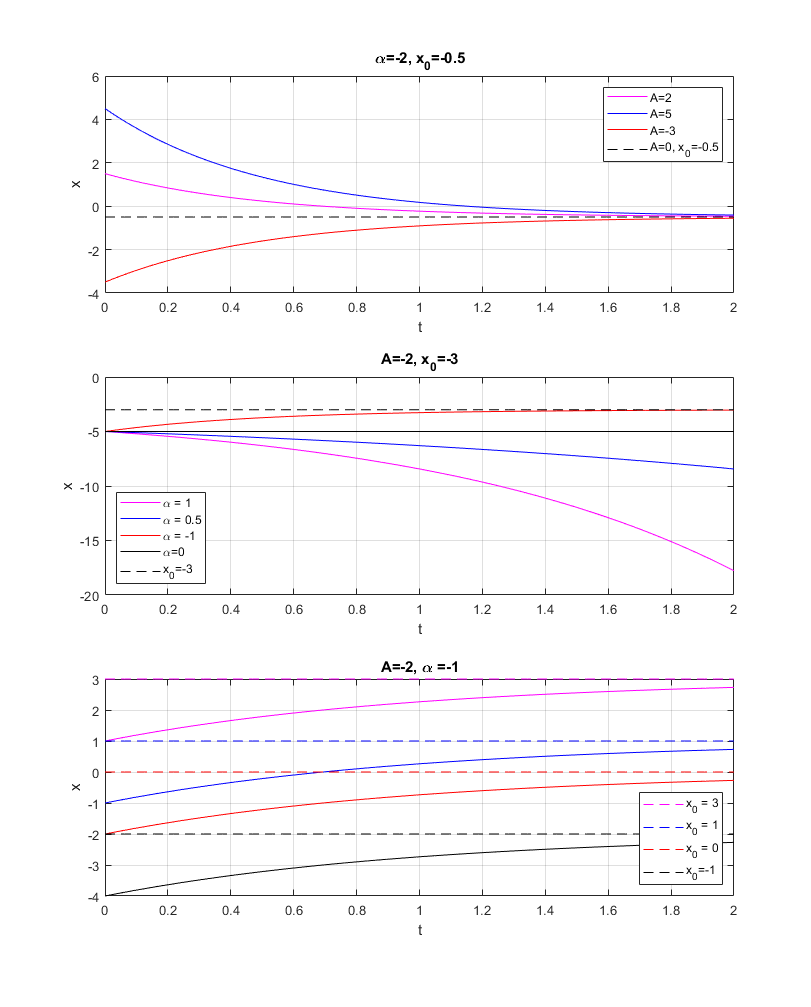
\includegraphics[width=0.8\textwidth]{a_graphs.png}
    \label{fig:my_label}
\end{figure}
\begin{flushleft}
Wnisoki:\\
Parametr $A$ nie ma wpływu na stabilność układu. Wpływa na to czy wkyres maleje czy rośnie w zależności od tego czy jest ujemny czy dodatni oraz gdzie spotyka się z osią pionową.\\
Parametr $\alpha$ wpływa na stabilnośc układu. Dla $\alpha > 0$ układ jest nie stabilny a dla $\alpha < 0 $ układ jest niestabilny.\\
Parametr $x_0$ nie wpływa na stabilość układu. Decydyuje o wartości na jakiej układ się ustabilizuje. Przesuwa wykres w górę lub w dół zależnie od wartości parametru.
\end{flushleft}
\subsection{$\alpha,\omega,\varphi$}
$$
x(t)=Ae^{\alpha t}cos(\omega t + \phi)+x_o
$$
\begin{figure}[h]
    \centering
    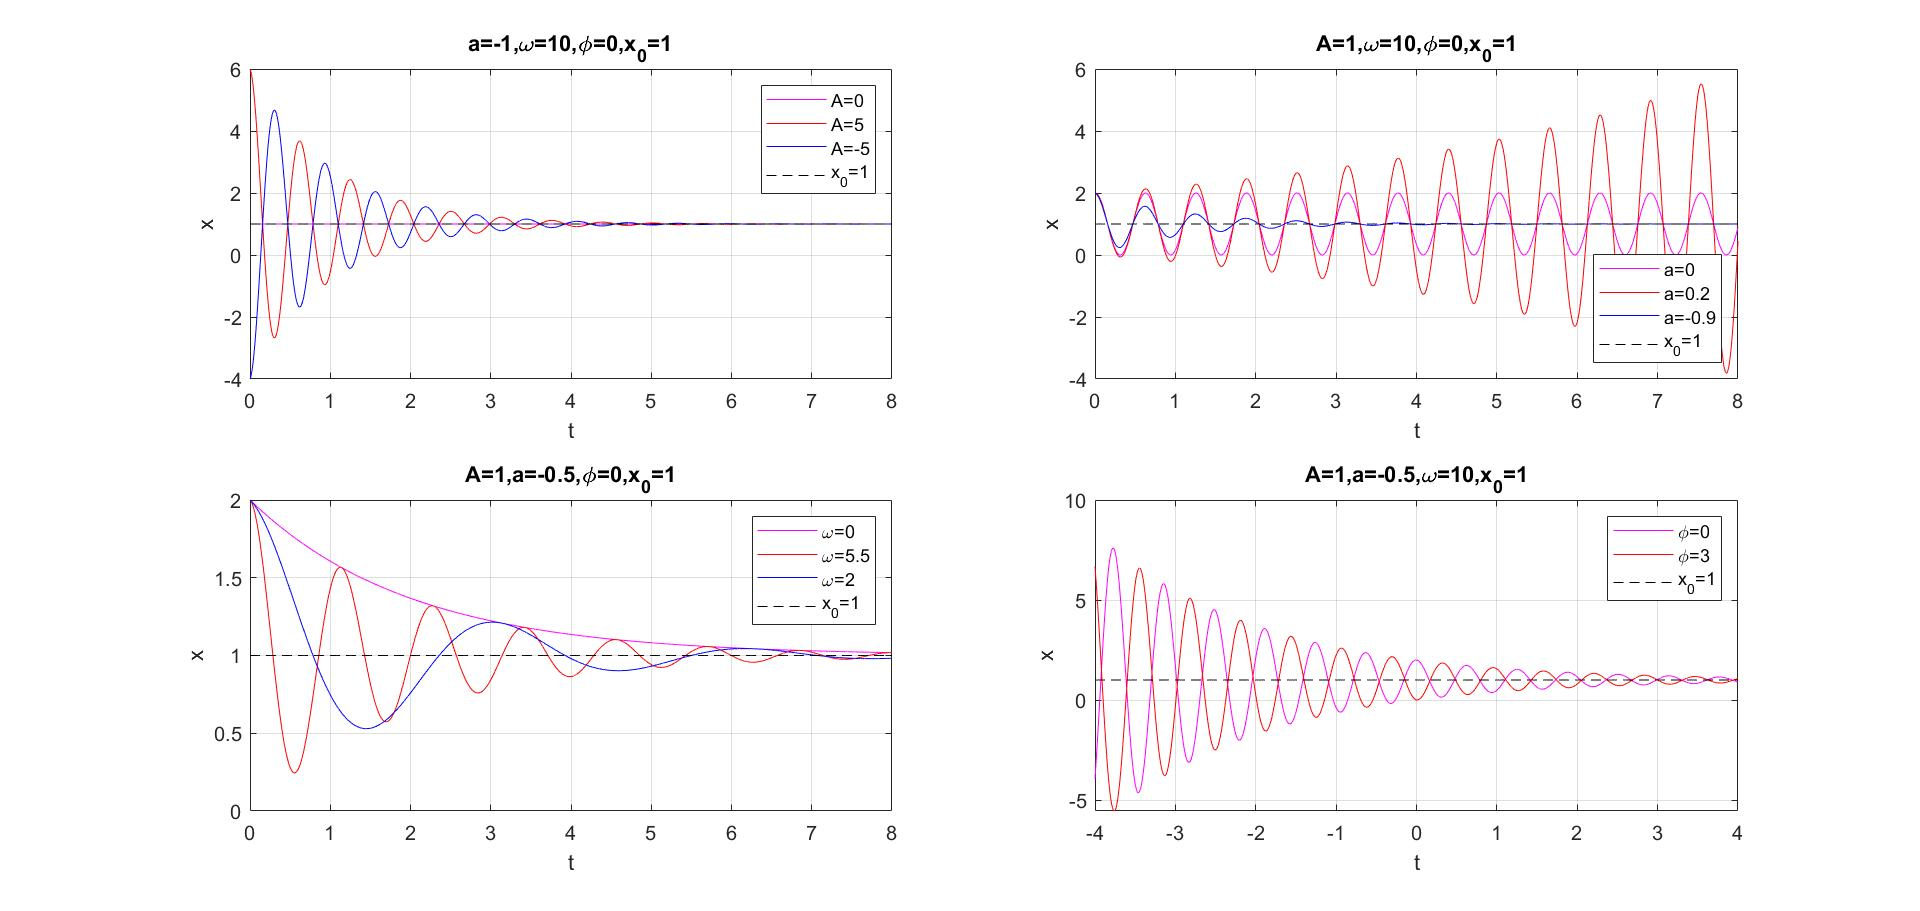
\includegraphics[width=1.2\textwidth]{b_wykresy.jpg}
    \label{fig:my_label}
\end{figure}
\begin{flushleft}
Wnioski:\\
Parametr $\alpha$ wpływa znacząco na zanikanie funkcji. Dla $\alpha < 0$ funkcja zanika do zera (układ się stabilizuje). Dla $\alpha > 0$ funkcja będzie uciekać od zera(układ jest nie stabilny).\\
Parametr $\omega$ wpływa na częstotliwośc oscylacji funkcji. Dla dużych $\omega$ oscylacje funkcji będą się pojawiać częściej funkcja będzie bardzije zagęszczona. \\
Parametr $\phi$ wpływa na przesunięcie fazowe funkcji. \\
\end{flushleft}
\subsection{$\alpha_i,A_i$}
a)
$$
x(t)=A_1e^{\alpha_1 t}+A_2e^{\alpha_2 t} + x_o
$$
Wnioski:\\
Sumowanie parametr $\alpha_i$ wpływa znacząco na to czy funkcja zanika. Dla dwuch parametrów $\alpha_i$ o ujemnych znakach funkcja zanika, lecz gdzy tylko jeden z parametrów $\alpha_i$ jest dodani to funkcja już nie zanika. \\
Sumowanie parametru $A_i$ jest bardzo intuicyjne. Gdy dwie skłądowe mają taki sam znak ich wpływ na kształt funkcji jest zsumowany. W rzypadku gdzie parametry $A_i$ mają różne znaki najbardziej znaczący jest ten któy ma większą wartość bezwzglęną.  \\
\newpage
\begin{figure}[h]
    \centering
    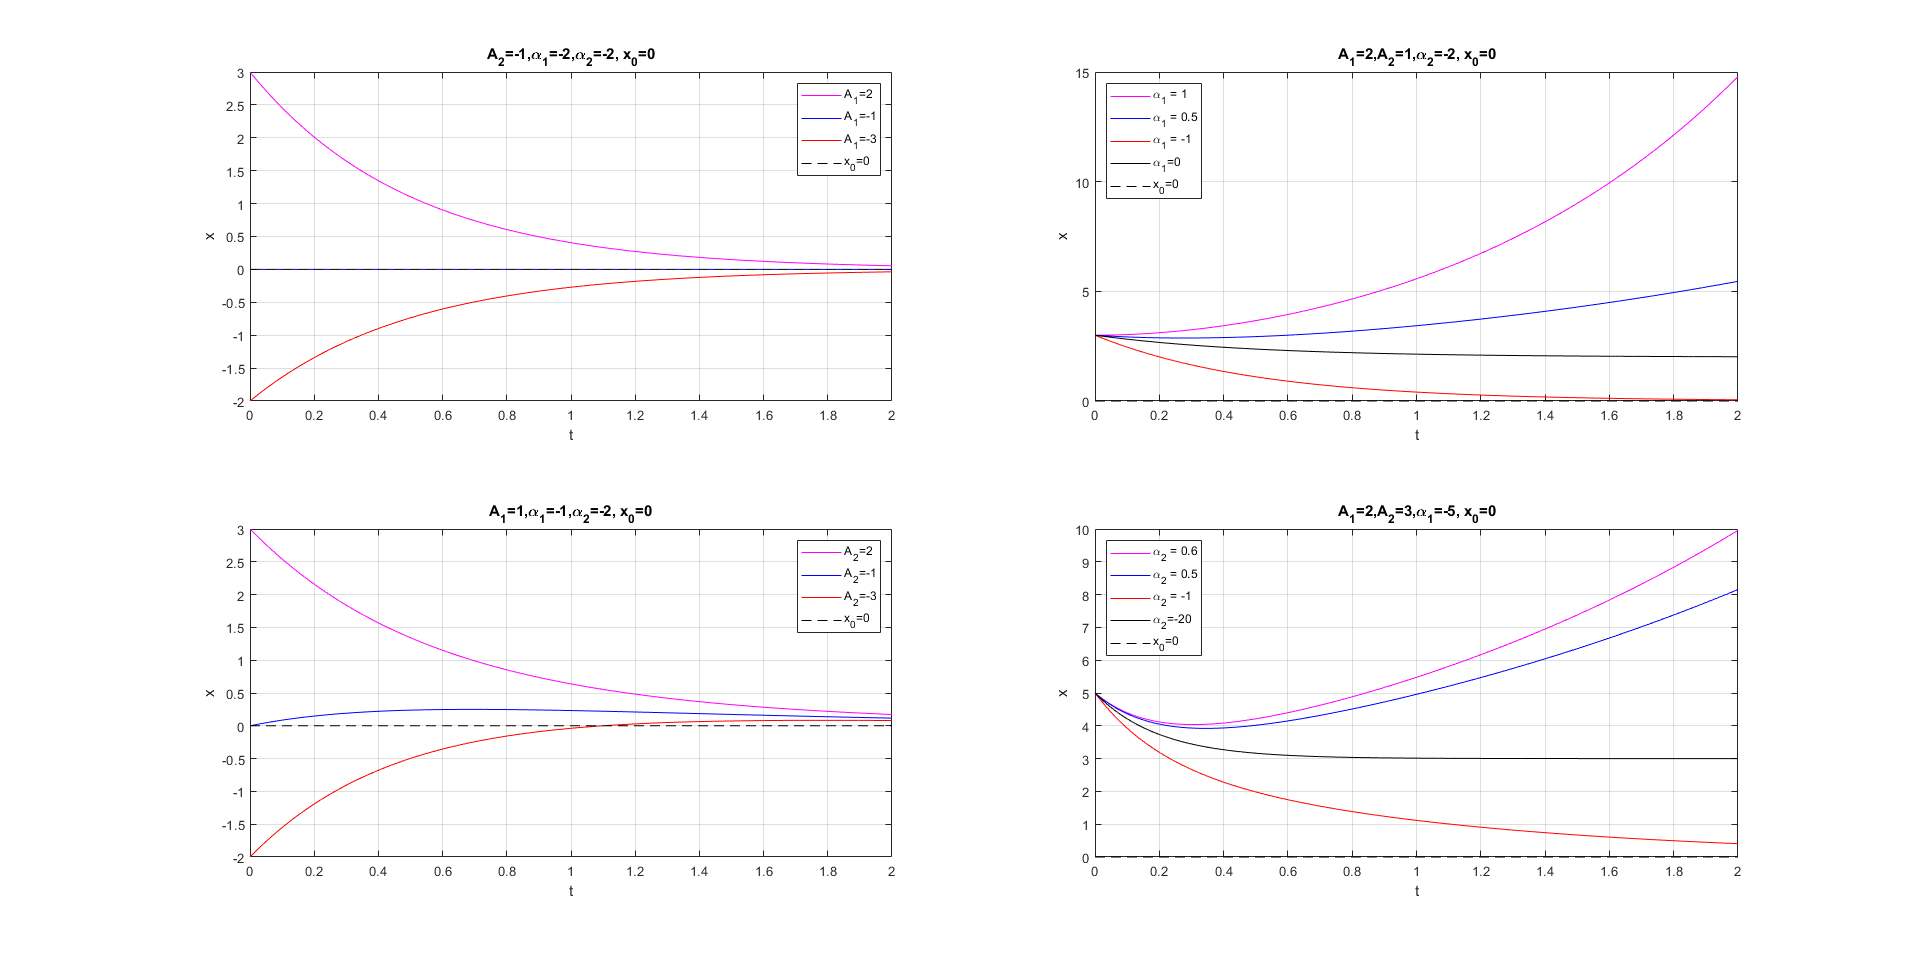
\includegraphics[width=1\textwidth]{c_graphs.png}
    \label{fig:my_label}
\end{figure}
b)
$$
x(t)=A_1e^{\alpha_1 t}+A_2e^{\alpha_2 t}cos(\omega t+\varphi)
$$
\begin{figure}[h!]
    \centering
    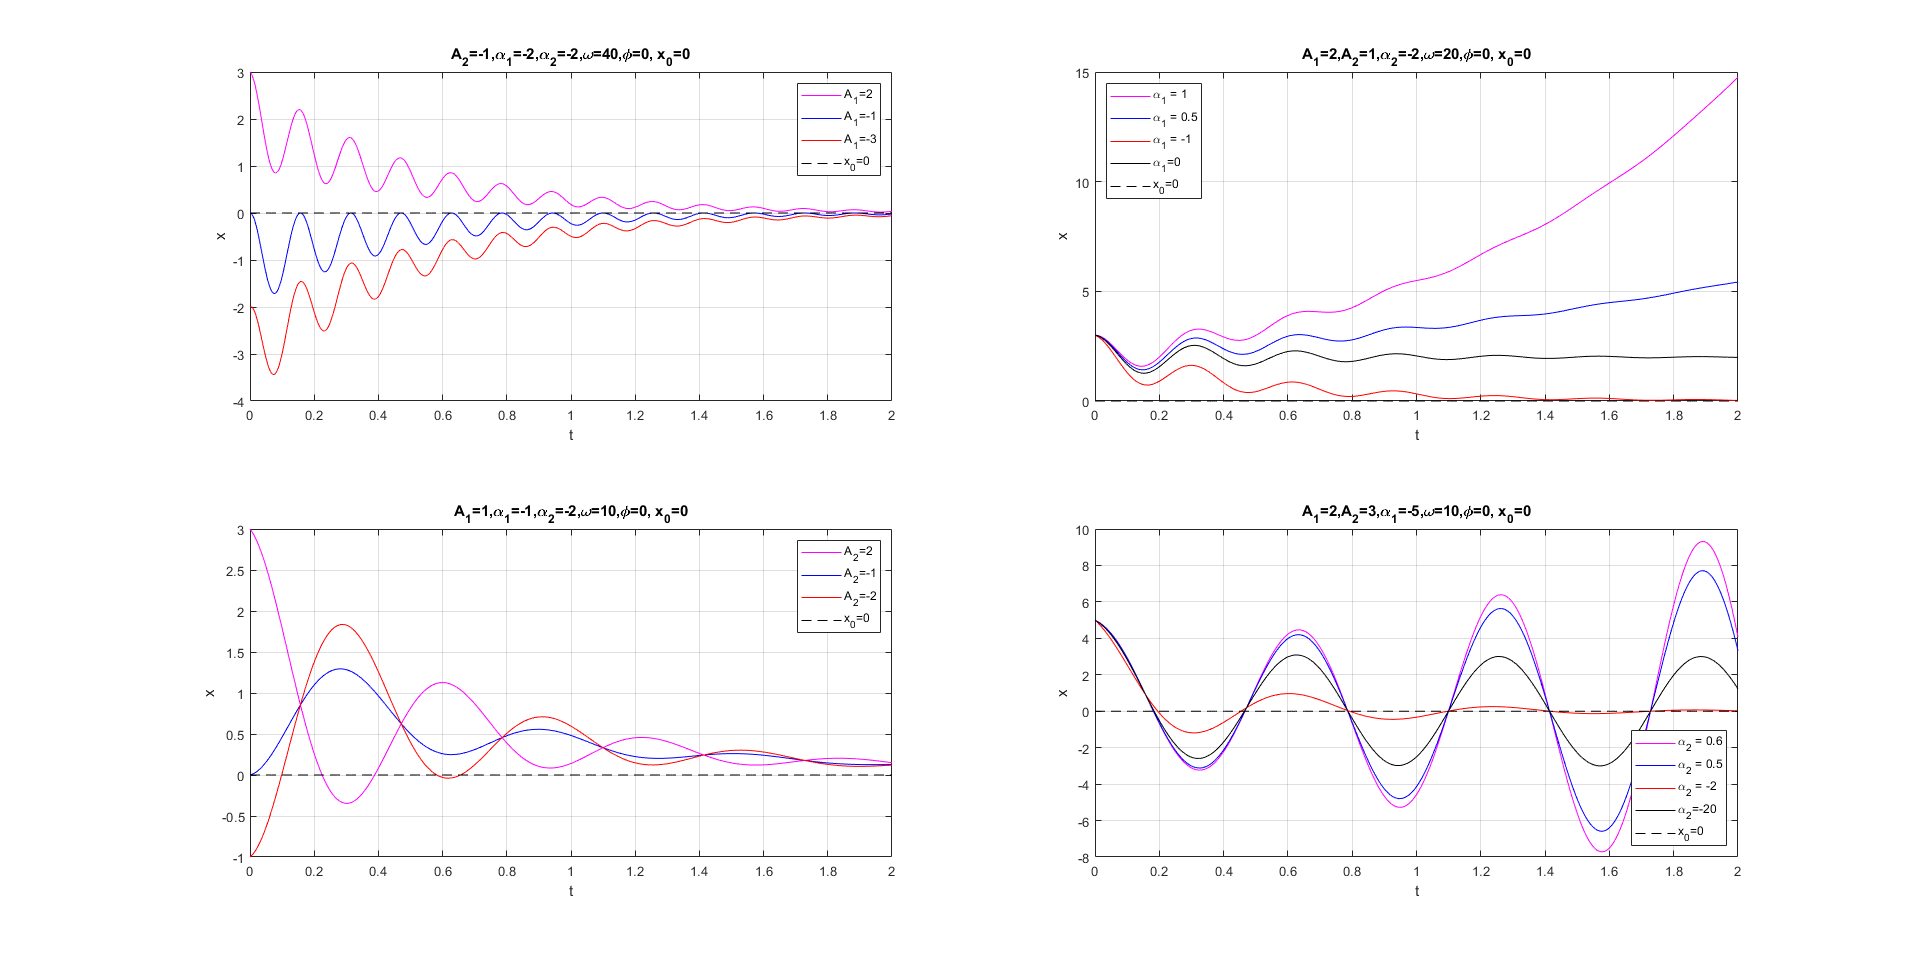
\includegraphics[width=1\textwidth]{d_graphs.png}
    \label{fig:my_label}
\end{figure}
\begin{flushleft}
Wnioski:\\
Sumowanie parametr $\alpha_i$ ma duży wpływ na to czy funkcja zanika. Dla dwuch parametrów $\alpha_i < 0 $ funkcja zanika, w sytuacji gdzie tylko jeden z parametrów $\alpha_i < 0$ a drugi parametr $\alpha_i > 0$ to funkcja nie zanika. \\
Sumowanie parametr $A_i$ w tej funkcji działa analogicznie do funkcji w podpunkcjie 3.3a. Jeśli znaki parametrów $A_i$ są takie same ich ewekt się 
dodaje, jeśli znaki parametró $A_i$ są różne to najważniejszy jest parametr z większą wartością bezwzględną.\\
\end{flushleft}



\section{Wnioski.}
Jak pokazały powyższe przykłady zanając jeden z parametrów funkcji możemy w mniejszym lub większym stopniu oszcacować jego wygląd. Można to przełożyć na ocenianie opisów modeli i w szybki sposób stwierdzić czy model się ustabilizuje czy nie, ponieważ niektóre parametry nie mają wpływu na to czy funkcja zanika do jakiejś wartości czy nie. 
\section{Załączniki.}
\begin{figure}[h!]
    \centering
    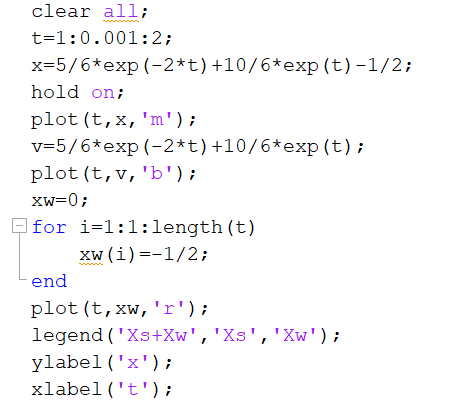
\includegraphics[width=0.5\textwidth]{kod1.png}
    \label{fig:my_label}
\end{figure}
\begin{figure}
    \centering
    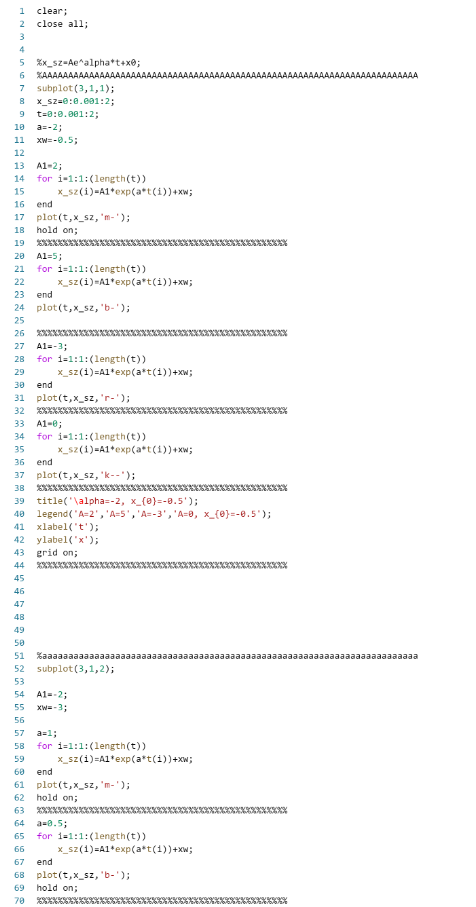
\includegraphics[width=0.7\textwidth]{a_1_m.png}
    \label{fig:my_label}
\end{figure}
\begin{figure}
    \centering
    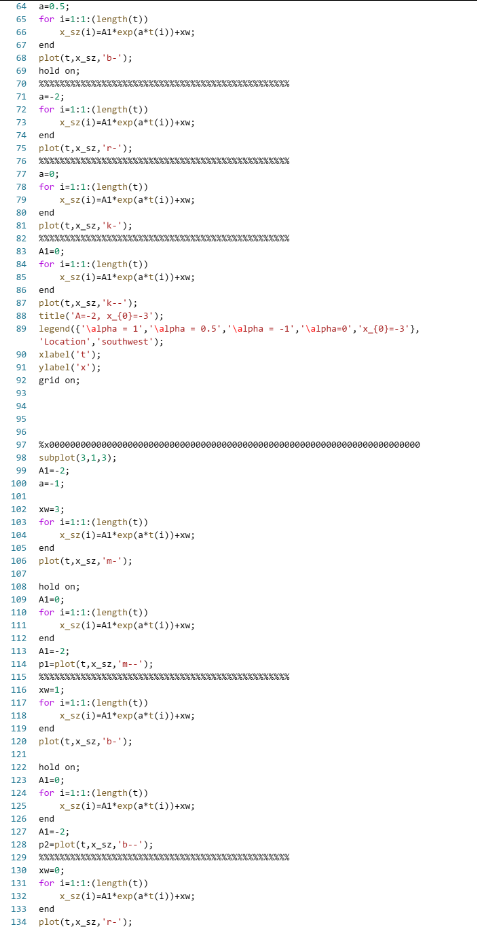
\includegraphics[width=0.7\textwidth]{a_2_m.png}
    \label{fig:my_label}
\end{figure}
\begin{figure}
    \centering
    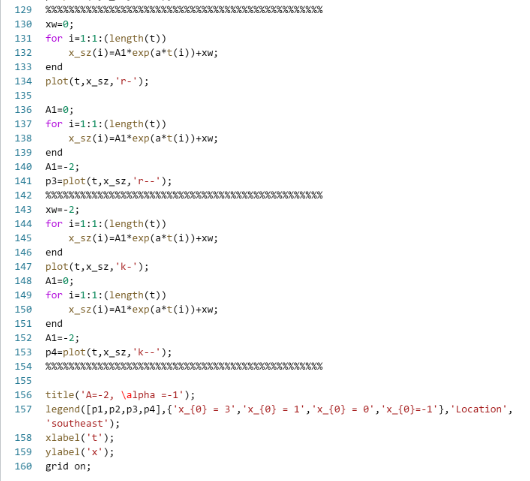
\includegraphics[width=0.7\textwidth]{a_3_m.png}
    \label{fig:my_label}
\end{figure}
\end{document}
